\begin{center}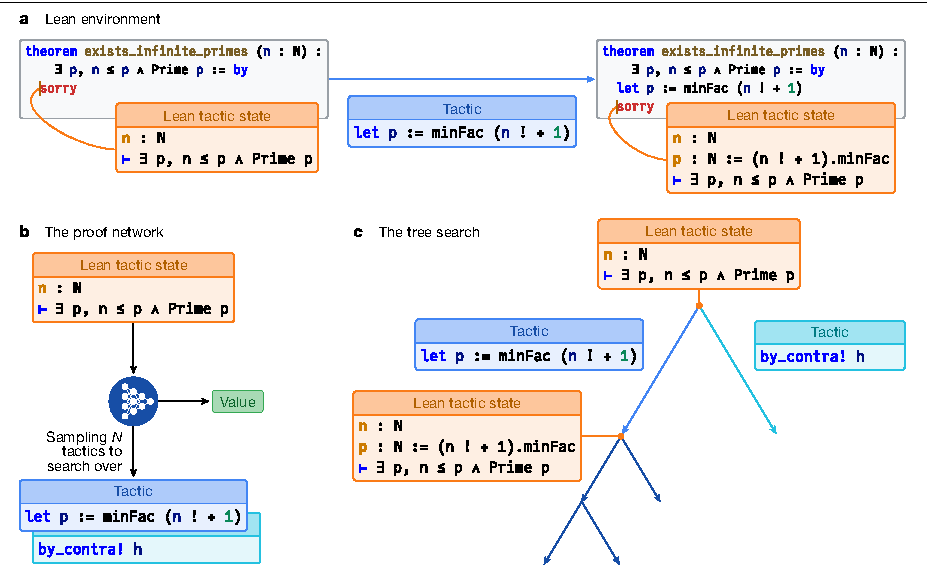
\includegraphics[width=\linewidth]{../papers/translations/alphaproof/assets/fig1.pdf}\end{center}
\phantomsection
\noindent\textbf{原文图 1. AlphaProof 的核心推理组成.}\paperlabel{1}{alphaproof-fig1}
a, 证明每一步所在的 Lean 环境. 智能体观测初始 Lean tactic 状态 (左), 描述待证定理. \texttt{sorry} 是 Lean 中表示证明未完成的占位符. 对环境应用一个 tactic, 例如原图的 \texttt{let p := minFac (n! + 1)}, 得到新状态, 可能引入新假设或改变目标 (右框). b, 证明网络以当前状态为输入, 输出 $N$ 个值得尝试的 tactic 和一个估计证明难度的价值. c, 树搜索使用这些输出探索可能证明路径: 从初始状态 (根) 开始迭代扩树, 每节点调用网络 (b), 生成有潜力的 tactic 与当前状态价值估计. 在环境 (a) 应用 tactic (边), 得新证明状态 (子节点). 网络价值智能指导搜索, 将计算集中于最有潜力路径, 例如更深入探索左分支.

\noindent\textbf{图中文字对应.} Lean environment: Lean 环境; Lean tactic state: Lean tactic 状态; Tactic: tactic; The proof network: 证明网络; The tree search: 树搜索; Value: 价值; Sampling $N$ tactics to search over: 采样 $N$ 个 tactic 供搜索. 所有 Lean 代码、$n,p$ 类型与假设、目标符号、分支和状态均以原图保留. 图中命题是对自然数 $n$ 寻找不小于 $n$ 的素数 $p$; \texttt{minFac} 为原代码的最小素因子操作名.
